\chapter{Image processing based on CUDA}

This chapter include the Image processing acceleration based on CUDA.

\section{Novel multi-scale retinex with color restoration on graphics processing unit}
\subsection{Abstract}
In this paper, a parallel application of the MSRCR+AL algorithm on a GPU is presented. For the various configurations in our test, the GPU-accelerated MSRCR+AL shows a scalable speedup as the resolution of an image increases. The up to $45 \times$ speed up $(1024 \times 1024)$ over the single-threaded CPU counterpart shows a promissing direction of using the GPU-based MSRCR+AL in large scale, time-critical applications. We also achieved 17 frames per second in video processing $(1280 \times 720)$. 

\subsection{Content}
In our implementation, the CUFFT provides a simple
interface for computing FFTs. After the plans of both
forward and inverse FFTs are created according to the
CUFFT requirements, the image data and the Gaussian
filters can be parallel transformed to frequency domain.
The multiplication between image data and Gaussian filters
in frequency domain is finished by ModulateandNormal-
ize() function, which is also provided by the CUFFT
library.

The atomic function atomicAdd() provided by
CUDA is used in the kernel histogram function to guar-
antee to be performed without interference from other
threads.
\subsection{Parallel optimization strage}
\subsubsection{size of thread block and grid}
For example, the maximum number of
threads on the lower capability version of CUDA is
512, but newer CUDA-enabled GPUs with 2.x computecapability can reach 1,024. But, each streaming multi-
processer (SM) can only execute 1,536 threads simul-
taneously. Therefore, we set the number of threads per
block at 192, which means each SM can fully execute
eight blocks to maximize resources.
\subsubsection{Memory access optimization}
A thread needs 400–600 clock cycles to access the
global memory, but only needs about 4 clock cycles to
access fast memory units such as register and shared
memory due to lower access latency. Therefore, taking
full advantage of the multi-level GPU memory storage
components can obtain quick data access to improve
the execution performance effectively.

\subsubsection{Loop unrolling}
After loop unrolling, the code only needs to run one time to
write the result. The number of write processes decreases
$66.7 \%$ compared with the serial code. Also, it only needs
one time to read the result, compared with three times had
we used in the serial code. The number of read processes
decreases $66.7 \% $ as well. Furthermore, this loop unrolling
strategy can be applied to sum different scale results
together for the Multi-scale Retinex. More importantly, in
the reduction algorithm for the summation process, this
strategy is used to greatly increase the calculation speed
and reduce the instruction overhead.
\subsection{Conclusion}
see the Abstract subsection.

\section{Image Convolution}
This section includes all articles I have read relating to Image Convolution using CUDA.
Image convolution is usually used in image filtering, like gaussian filter.
\subsection{Na\"ive  Implementation}
From the idea of convolutio filter itself, the most naive approach is to use global memory to send data to device and each thread accesses this to compute convolution kernel. Our convolution kernel size is radius 8 (total $17 \times 17$ multiplicaiton for single pixel value). In image border area, reference value will be set to 0 during computation. This naive approach includes many of conditional statements and this causes very slow execution.
\begin{figure}[!hbtp]
\centering
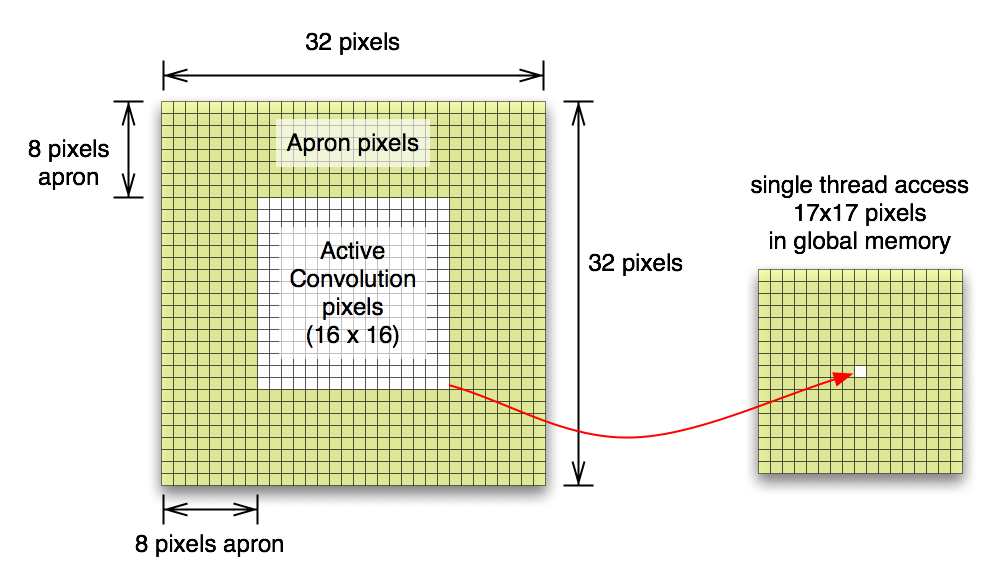
\includegraphics[width=0.8\textwidth]{CUDAImageProcessing/ImageConvoOnGlobal}
\caption{Image Convolution based on Global Memory}
\label{fig3.1}
\end{figure}
The code is as shown below:

\lstdefinestyle{customCpp}{
 belowcaptionskip=1\baselineskip,
  breaklines=true,
%  frame=L,
  xleftmargin=\parindent,
  language=C,
  showstringspaces=false,
  basicstyle=\footnotesize\ttfamily,
  keywordstyle=\bfseries\color{green!40!black},
  commentstyle=\itshape\color{purple!40!black},
  identifierstyle=\color{blue},
  stringstyle=\color{orange},
}

\lstset{style=customCpp,caption={Image Convolution based on global memory}}
\lstinputlisting{CUDAImageProcessing/filterGlobal.cu}

For $396 \star 396$ input image, the time is 1.6ms.
When the input filter is stored in constant memory or specified by {\color{red}{'\_\_restrict\_\_'}}, the time is 1.7 or 1.8 ms.

\subsection{Na\"ive Shared Memory Implementation}
The simplest approach to implement convolution in CUDA is to load a block of the
image into a shared memory array, do a point-wise multiplication of a filter-size portion of
the block, and then write this sum into the output image in device memory. Each thread
block processes one block in the image. Each thread generates a single output pixel.

The algorithm itself is somewhat complex. For any reasonable filter kernel size, the
pixels at the edge of the shared memory array will depend on pixels not in shared memory.
Around the image block within a thread block, there is an \textit{apron} of pixels of the width of the
kernel radius that is required in order to filter the image block. Thus, each thread block
must load into shared memory the pixels to be filtered and the apron pixels.

Note: The apron of one block overlaps with adjacent blocks. The aprons of the
blocks on the edges of the image extend outside the image – these pixels can either be
clamped to the color of pixels at the image edge, or they can be set to zero.

\begin{figure}[!hbtp]
\centering
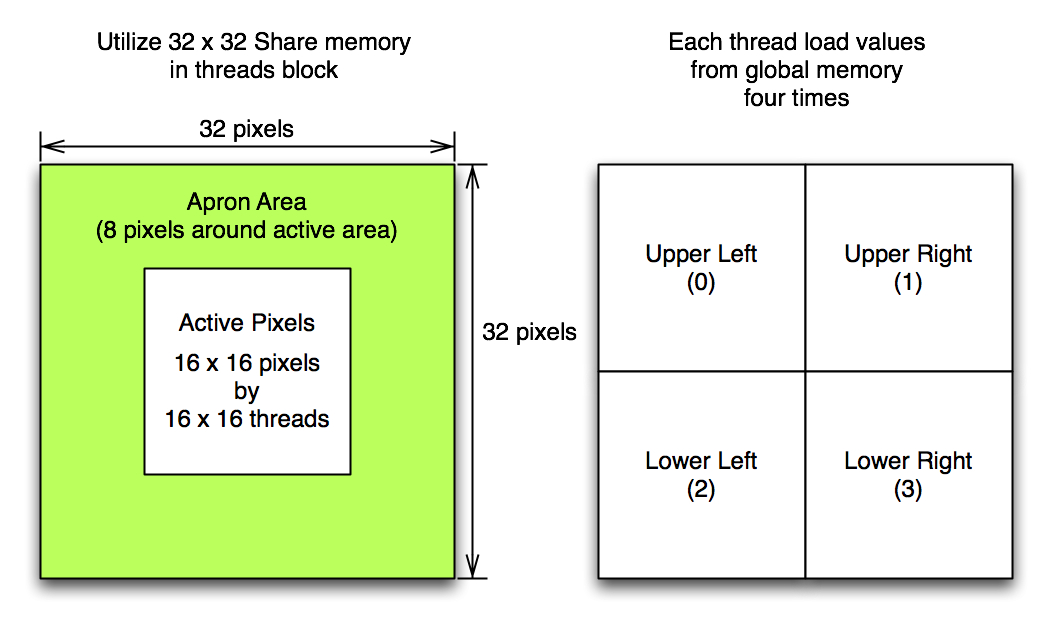
\includegraphics[width=0.9\textwidth]{CUDAImageProcessing/ImageConvoOnShare1}
\caption{Image Convolution based on shared memory}
\label{fig3.2}
\end{figure}

The first attempt was to keep active thread size as same as previous and increase block size for apron pixels. This did not work since convolution kernel radius is 8 and it make block size to $32 \times 32$ (1024). This is bigger than G80 hardware limit (512 threads max per block).

Therefore, I changes scheme as all threads are active and each thread loads four pixels and keep the block size $16 \times 16$. Shared Memory size used is $32 \times 32$ (this includes all necessary apron pixel values for $16 \times 16$ active pixels). Below shows quite a bit of performance improve. This is almost $\times2.8$ speed up over naive approach (in 2048 resolution).

\lstset{style=customCpp, caption={Image colvotion based on Shared memory and Apron}}
\lstinputlisting{CUDAImageProcessing/filterShare.cu}

Note : the value \verb|“gLoc - KERNEL_RADIUS - IMUL(dataW, KERNEL_RADIUS)”| is the shift address of the image data on the upper left corner.
在本方法中,主要是索引的问题,所以又分为Share Memory的索引 以及 图像数据的索引。在具体实现过程中,选择是固定thread Block的大小,同时在share memory中添加边界。所以将图像数据拷贝到Share Memory中时,分了四次,分别对应:左上角,右上角,左下角、右下角。也就是图\ref{fig3.2}中的对应关系,其处理过程就是将小的图像块映射到大的Share memory中,从这个方面进行理解。

\subsection{Separable Gaussian Filtering}
\subsubsection{Separable Convolution}
A tow-dimensional filter s is said to be separable if it can be written as the convolution of tow one-dimesional filters \textit{\textbf{v}} and \textit{\textbf{h}}:
\begin{displaymath}
s = v * h
\end{displaymath}
''How to determine if a matrix is an outer product of two vectors?''\\
''Go look at the \textbf{rank} function. ''.
Of course. If a matrix is an outer product of two vectors, its rank is 1. 

So the test is this: The rank of A is the number of nonzero singular values of A, with some numerical tolerance based on eps and the size of A.

So how can we determine the outer product vectors? The answer is to go back to the svd function. Here's a snippet from the doc:

$[U, S, V] = svd(X)$ produces a diagonal matrix S of the same dimension as X, with nonnegative diagonal elements in decreasing order, and unitary matrices \textit{\textbf{U}} and \textit{\textbf{V}} so that
$X = U * S * V'$

A rank 1 matrix has only one nonzero singular value, so $X = U * S * V'$ becomes $U(:, 1) * S(1, 1) * V(:,1)$. This is basically the outer product we were seeking. Therefore, we want the first columns of \textit{\textbf{U}} and \textit{\textbf{V}}. (We have to remember also to use the nonzero singular value as a scale factor.)

\subsubsection{Seperate Gaussian filter}
First chose, somewhat artitrarily to split the scale factor, S(1, 1), "equally" between \textit{\textbf{v}} and \textit{\textbf{h}}. Except for normal floating-point roundoff differences, gaussian and v*h are equal. Just show as following : 
\begin{displaymath}
\begin{gathered}
\left[ U, S, V \right]= svd(X)\\
v = U(:, 1) * sqrt(S(1, 1))\\
h = V(:, 1)‘ × sqrt(S(1, 1))\\
GassianFilter = v * h
\end{gathered}
\end{displaymath}
More details can be found at :\href{http://blogs.mathworks.com/steve/2006/11/28/separable-convolution-part-2/}{Separable Convolution}.

\subsection{Optimizing for memory coalescence}
Base read/write addresses of the warps of 32 threads also must meet half-warp
alignment requirement in order to be coalesced. If four-byte values are read, then the base
address for the warp must be 64-byte aligned, and threads within the warp must read
sequential 4-byte addresses. If the dataset with apron does not align in this way, then we
must fix it so that it does.

The approach used in the row filter is to have additional threads on the leading edge
of the processing tile, in order to make threadIdx.x == 0 always reading properly aligned
address and thus to meet global memory alignment constraints for all warps. This may seem
like a waste of threads, but it is of little importance when the data block, processed by a
single thread block is large enough, which decreases the ratio of apron pixels to output
pixels.

Each image convolution pass in both row and column pass is separated into two
sub stages within corresponding CUDA kernels. The first stage loads the data from global
memory into shared memory, and the second stage performs the filtering and writes the
results back to global memory. We mustn’t forget about the cases when row or column
processing tile becomes clamped by image borders, and initialize clamped shared memory array indices with correct values. Indices not lying within input image borders are usually
initialized either with zeroes or with values, corresponding to clamped image coordinates. In
this sample we opt for the former.

In between the two stages there is a \textbf{\_\_syncthreads( )} call to ensure that all threads
have written to shared memory before any processing begins. This is necessary because
threads are dependent on data loaded by other threads.

For both the loading and processing stages each active thread loads/outputs one
pixel. In the computation stage each thread loops over a width of twice the filter radius plus
1, multiplying each pixel by the corresponding filter coefficient stored in constant memory.
Each thread in a half-warp accesses the same constant address and hence there is no penalty
due to constant memory bank conflicts. Also, consecutive threads always access consecutive
shared memory addresses so no shared memory bank conflicts occur as well.

The column filter pass operates much like the row filter pass. The major difference
is that thread IDs increase across the filter region rather than along it. As in the row filter
pass, threads in a single half-warp always access different shared memory banks, but the
calculation of the next/previous addresses involves increment/decrement by
COLUMN\_TILE\_W, rather than simply 1. In the column filter pass we do not have inactive
“coalescing alignment” threads during the load stage, because we assume that the tile width
is a multiple of the coalesced read size. In order to decrease the ratio of apron to output
pixels we want image tile to be as tall as possible, so to have reasonable shared memory
utilization we shoot for as thin image tiles as possible: 16 columns.

\section{CUDA C Best Practice Guide}
\subsection{Performance Metrics}
\subsubsection{Timing}
\begin{itemize}
\item Using CPU Timers \\
	Should call \textit{cudaDeviceSynchronize()} immediately before starting and stopping the CPU timer.
\item Using CUDA GPU Timers\\
	The device will record a timestamp for the event when it reaches that event in the stream. This value is expressed in milliseconds and has a resolution of approximately half a microsecond.
\end{itemize}
\subsubsection{Bandwidth}
Bandwidth - the rate at which data can be transferred - is one of the most important gating factors for performance.


\section{Npp Library Image Filters}
\subsection{Image Data}
\subsubsection{Line Step}
All image data passed to NPPI primitives requires a line step to be provided. It is important to keep in mind that this line step is always specified in terms of bytes, not pixels.

\section{PTX ISA 6.0}
\subsection{PTX Machine Model}
The \textit{Multiprocessor} maps each thread to one \textit{scalar processor} core, and each scalar thread executes independently with its own instruction address and register state.

Individual threads composing a SIMT warp start together at the same program address but are otherwise free to branch and execute independently. A warp executes one common instruction at a time, so full efficiency is realized when all threads of a warp agree on their execution path. If threads of a warp diverge via a data-dependent
conditional branch, the warp serially executes each branch path taken, disabling threads that are not on that path, and when all paths complete, the threads converge back to the same execution path. 

Each multiprocessor has \textbf{on-chip memory} of the four following types : 
\begin{itemize}
\item Local 32-bit registers per processor;
\item Shared memory (parallel data cache);
\item Read-only \textit{constant cache} that is shared by all scalar processor cores;
\item Read-only \textit{texture cache} 
\end{itemize}

The local and global memory spaces are read-write regions of \textbf{device memory} and are not cached.

If there are not enough registers or shared memory available per multiprocessor to process at least one block, the kernel will fail to launch.

\subsubsection{Syntax}
PTX programs are a collection of text source modules(files). PTX source modules have an assembly-language style syntax with instruction operation codes and operands. Pseudo-operations specify symbol and addressing management. The \textit{ptxas}
optimizing backend compiler optimizes and assembles PTX source modules to produce
corresponding binary object files.
\subsubsection{Source Format}
PTX is case sensitive and uses lowercase for keywords.

Each PTX module must begin with a \textbf{.version} directive specifying the PTX language version, followed by a \textbf{.target} directive specifying the target architecture assumed. 

\subsubsection{Statements}
A PTX statement is either a \textbf{directive} or an \textbf{instruction}. Statements begin with an optional label and end with a semicolon.
\begin{itemize}
\item Directive Statements \\
Directive keywords begin with a dot, so no conflict is possible with user-defined
identifiers. 如图\ref{PTXDirectives}所示。
\begin{figure}[!htbp]
\centering
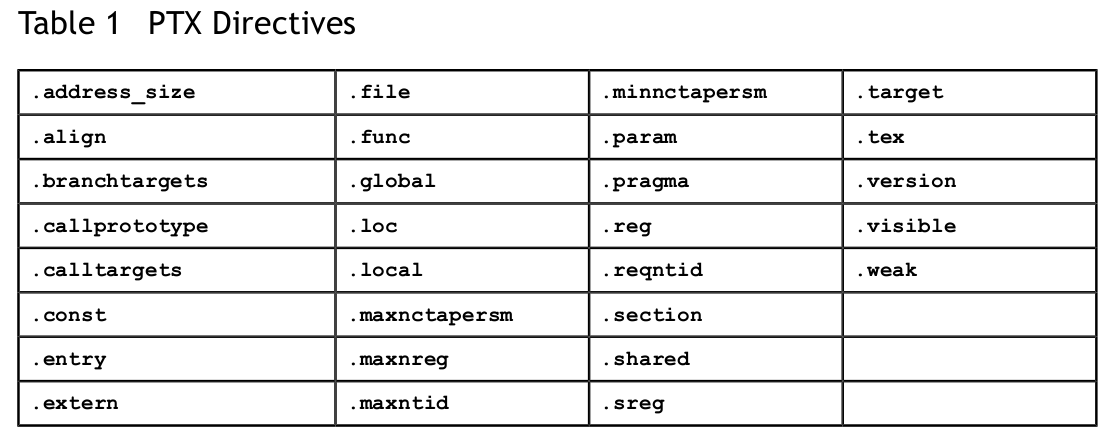
\includegraphics[width=0.9\textwidth]{CUDAImageProcessing/PTXDirectives}
\caption{PTX Directives}
\label{PTXDirectives}
\end{figure}
%\begin{table}[!htbp]
%\begin{tabular}{c|c|c}
%\hline
%A & B & C \\
%\hline
%\end{tabular}
%\end{table}
\item Instruction Statements \\
Instructions are formed from an instruction opcode followed by a \textbf{comma-separated} list
of zero or more operands, and terminated with a semicolon.

Operands may be register
variables, constant expressions, address expressions, or label names.
The guard predicate
follows the optional label and precedes the opcode, and is written as \textbf{@p} , where p is a
predicate register. The guard predicate may be optionally negated, written as \textbf{@!p}.

The destination operand is first, followed by source operands.
如图\ref{ReservedInstructionKeywords}所示。
\begin{figure}[!hbtp]
\centering
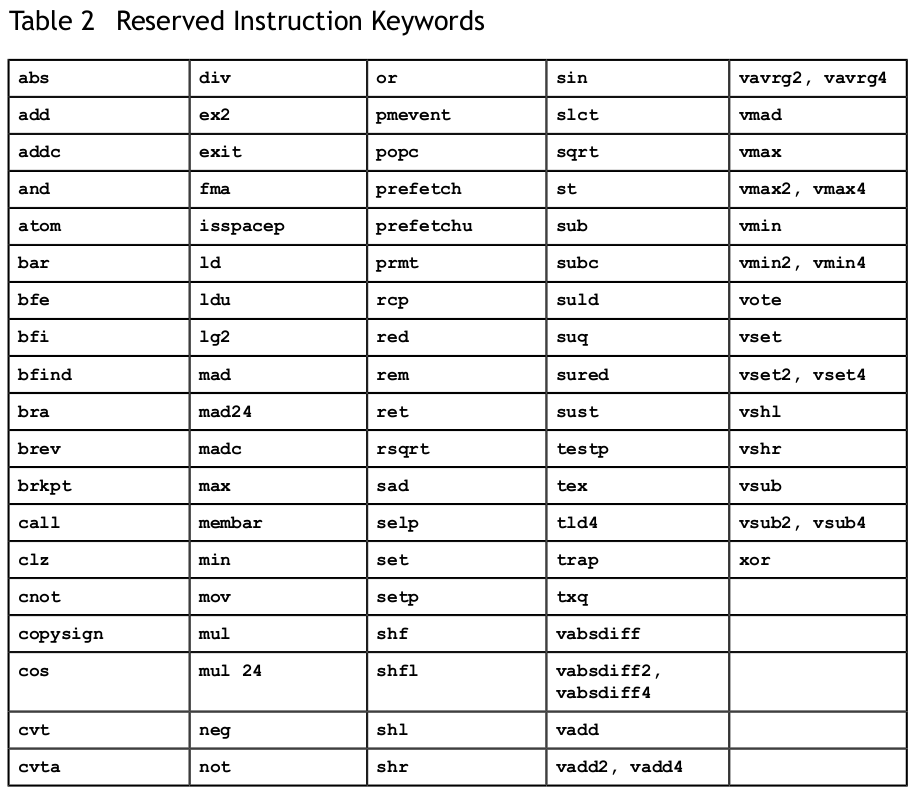
\includegraphics[width=0.9\textwidth]{CUDAImageProcessing/ReservedInstructionKeywords}
\caption{Reserved Instruction Keywords}
\label{ReservedInstructionKeywords}
\end{figure}


\end{itemize}


